\documentclass[11pt]{article}
\usepackage[margin=2cm]{geometry}
\usepackage[portuguese]{babel}
\usepackage[utf8]{inputenc}
\usepackage{hyperref}
\usepackage{indentfirst}
\usepackage{subfig}
\usepackage{listings}
\usepackage{color}

\definecolor{dkgreen}{rgb}{0,0.6,0}
\definecolor{gray}{rgb}{0.5,0.5,0.5}
\definecolor{mauve}{rgb}{0.58,0,0.82}

\lstset{frame=tb,
  language=R,
  aboveskip=3mm,
  belowskip=3mm,
  showstringspaces=false,
  columns=flexible,
  basicstyle={\small\ttfamily},
  numbers=none,
  numberstyle=\tiny\color{gray},
  keywordstyle=\color{blue},
  commentstyle=\color{dkgreen},
  stringstyle=\color{mauve},
  breaklines=true,
  breakatwhitespace=true,
  tabsize=3
}

\urlstyle{same}
\pagenumbering{arabic}
%\usepackage{multicol}
\hypersetup{
    colorlinks=true,
    linkcolor=black,
    filecolor=magenta,      
    urlcolor=blue,
    citecolor=black,
}
\usepackage[backend=bibtex]{biblatex}
\usepackage{graphicx}
\pagestyle{plain}

\newcommand{\gaspar}{Diogo Gaspar, 99207}

\begin{document}
\begin{center}
{\huge{Exercício 1 - Projeto Computacional PE 2022}} \\
\vspace{1.5mm}
{\large{\gaspar}} \\
\end{center}

\section{Descrição do Problema e da Solução}
O objetivo deste exercício é representar, através de um diagrama de barras, a produção de \textit{resíduos per capita} nos países \texttt{IT- Italia}, \texttt{UK - Reino Unido} e \texttt{GR - Grecia}, nos anos 2004 e 2018.

\vspace{0.5mm}
Para tal, recorreu-se ao seguinte trecho de código \texttt{R} (utilizando as bibliotecas \texttt{openxlsx, ggplot2, gridExtra} e \texttt{dplyr}):

\begin{lstlisting}
df <- read.xlsx("ResiduosPerCapita.xlsx", sheet = 1, rows = seq(11, 43), cols = seq(1, 3))
df <- rename(df, "Países" = "Anos", "Resíduos_per_Capita" = "┴.2018")
df <- df[df$"Países" %in% c("IT - Itália", "UK - Reino Unido", "GR - Grécia"), ]
# we need 6 rows (3 for each year)
df <- rbind(df, df)
df$"Ano" <- rep(c("2004", "2018"), each = 3)
# copy 2004 residue data to "Resíduos_per_Capita"
df[1:3, "Resíduos_per_Capita"] <- df[1:3, "2004"]
df <- df[, !(colnames(df) %in% c("2004"))] # drop the "2004" column

ggplot(df, aes(x = Países, y = Resíduos_per_Capita, fill = Ano)) + 
  geom_bar(stat = "identity", position = position_dodge()) + 
  theme_minimal() +
  labs(x = "Países", y = "Resíduos per Capita") +
  ggtitle("Resíduos per Capita em Itália, Reino Unido e Grécia nos anos 2004 e 2018")
\end{lstlisting}

O gráfico produzido pela chamada a \texttt{ggplot} é o seguinte:

% enter image from ../imgs/exercise-1.png
\begin{figure}
    \centering
    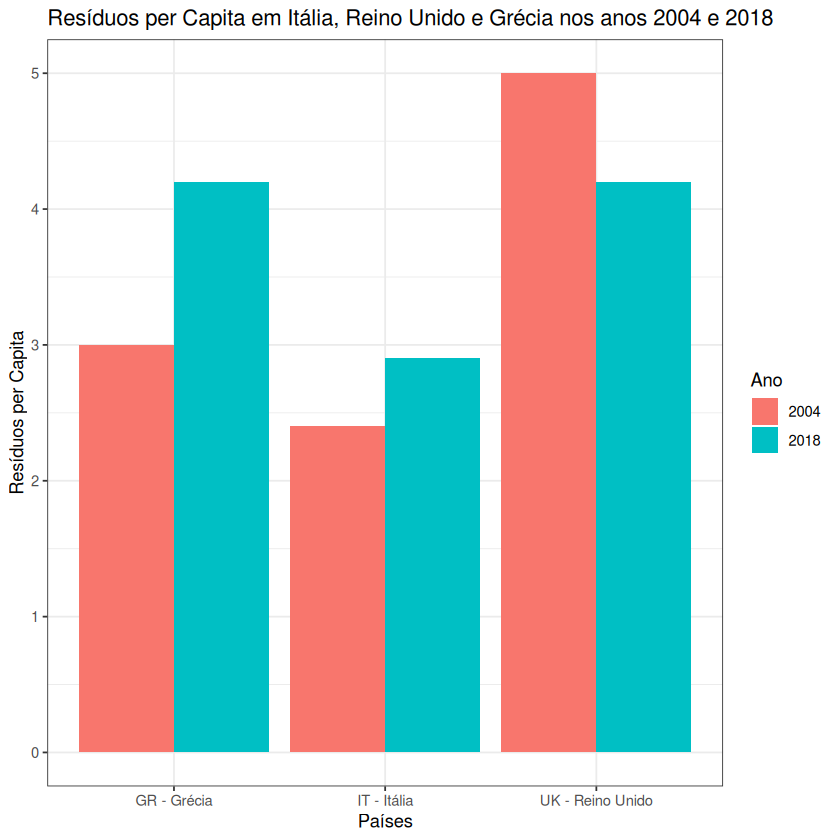
\includegraphics[width=10cm]{../imgs/exercise-1.png}
    \caption{Gráfico da produção de resíduos per capita nos países Itália, Reino Unido e Grécia nos anos 2004 e 2018}
    \label{fig:exercise-1}
\end{figure}

\end{document}